\section{Durchführung}
\label{sec:Durchführung}
Der Versuch wird wie in der Abbildung \ref{fig:aufd} dargestellten Schaltskizze aufgebaut.
\begin{figure}
    \centering
    \caption{Schaltplan zur Untersuchung einer Franck-Hertz-Kurve.\cite{v601}}
    \label{fig:aufd}
    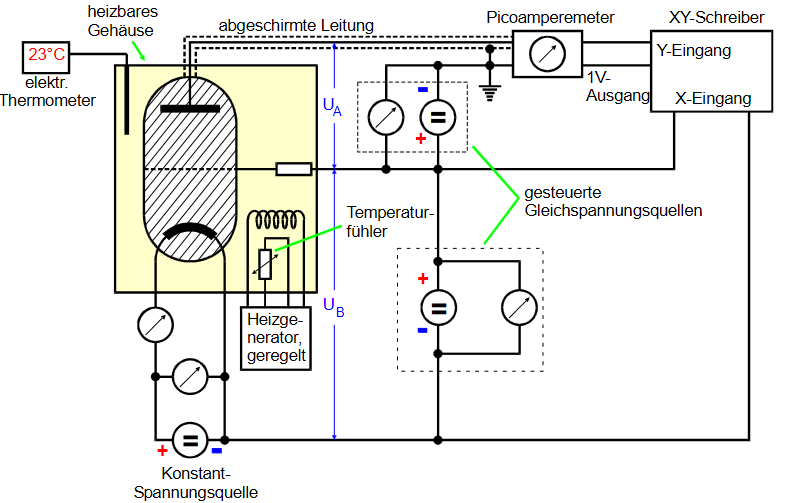
\includegraphics[width = 0.6 \textwidth]{pics/aufd.png}
\end{figure}
Zusätzlich zu den vorher beschriebenen Elektroden im Vakuumglas werden ein Heizgenerator, Temperaturfühler und ein Picoamperemeter zur Aufnahme der Franck-Hertz-Kurven verwendet.
Dabei ist das Amperemeter eine Alternative zu dem in Abbildung \ref{fig:aufd} dargestellten XY-Schreibers. 
\\
Zunächst wird die integrale Energieverteilung der beschleunigten Elektronen gemessen. Dazu wird 
$I_\text{A}$ in Abhängigkeit von $U_\text{A}$ gemessen, wobei eine konstante Bremsspannung $U_\text{B} = \SI{11}{\volt}$ angelegt ist. Diese Messung wird einmal
bei Raumtemperatur $T= \SI{26}{\celsius}$ und einmal nach Aufheizen auf $T=\SI{140}{\celsius}$ durchgeführt. 
Die Messung bei Raumtemperatur erfolgt in $U_\text{A}=\SI{1}{\volt}$ Schritten bis hin zum Maximalwert $U_\text{A}=\SI{10}{\volt}$.
Für die Messung bei $T=\SI{140}{\celsius}$ werden $U_\text{A}=\SI{0.5}{\volt}$ Schritte gewählt bis hin zum Maximalwert $U_\text{A}=\SI{6}{\volt}$.
\\
Danach werden drei Franck-Hertz-Kurven für konstantes $U_\text{A}=\SI{1}{\volt}$ und verschiedene Temperaturen $\SI{160}{\celsius} \geq T \geq \SI{200}{\celsius}$
entnommen. Es werden Wertepaare von $I_\text{A}$ und $U_\text{B}$ aufgenommen. Dabei wird die Beschleunigungsspannung erhöht bis fünf Maxima durchlaufen sind.